\section{Strålning genom fönster}

Solstrålning genom fönster orsakar snabba temperaturökningar i inomhusklimatet. Hur snabba och stora dessa temperaturökningar blir beror på en mängd parametrar varav de viktigaste omfattas av fönstrets utformning, det vill säga glasets reflektivitet och emmissitivitet, strålningens infallsvinkel som beror av tid på dagen och året och ytorna inomhus som solstrålningen faller på, så som persienner, gardiner, vägger och möbler. Fönstrets reflexivitet och emmisivitet är beror av solens infallsvinkel.

%\begin{itemize}
%\item{
%fönstrets utformning, det vill säga glasets reflektivitet och emmissitivitet.
%}
%\item{
%vinkeln relativt fönstret som strålningen infaller vid, det vill säga tid på dagen och året. Detta är starkt förknippat med föregående punkt. 
%}
%\item{
%de inomhus belägna ytorna som solstrålningen faller på, det vill säga persienner, gardiner, väggar, möbler, etcetera.
%}
%\end{itemize} 

\subsection{g-värden}\label{gvalue}

För att ange transmittansen av solstrålning genom fönster brukar man använda vad som kallas för g-värden (ibland även kallat ''Solar Factor''). Detta värde, mellan noll och ett, anger hur mycket av infallande solstrålnings normalprojektion som släpps igenom. Men eftersom ett sådant värde också beror på strålningens infallsvinkel (på grund av ökande reflektion med ökande vinkel) är den ofta svår att beräkna.

Enligt \cite{karlssonroos99} förändras detta vinkelberoende främst med antalet glas (flerglasfönster) samt typ av eventuella beläggningar på glaset. I samma artikel visades också att g-värdenas vinkelberoende kan approximeras med ett polynom

\begin{equation}\label{eq:radiationwindowstheory:gvalue}
g = g_0 \left( 1 - az^{\alpha} - bz^{\beta} - cz^{\gamma} \right)
\end{equation}

där $g_0$ är g-värdet då strålningen infaller vinkelrätt mot ytan, $a+b+c=1$ och $z=\theta/90$ då $\theta$ är vinkeln, mätt i grader, mellan fönstrets normal och solstrålningens riktning. Koefficienterna och exponenterna i \eqref{eq:radiationwindowstheory:gvalue} beror på typen av fönster, och i \cite{karlssonroos99} har empiriska undersökningar lett till aproximationen

\begin{align}\label{eq:gconstants}
a & = 8, & b & = 0.25/q, & c & = (1-a-b) \nonumber \\
\alpha & = 5.2 + 0.7q, & \beta & = 2, & \gamma & = (5.26+0.06p) + (0.73+0.04p)q
\end{align}

där p är antalet rutor i fönstret (treglasfönster medför $p = 3$) och q är en parameter, $1 \le q \le 10$, som varierar beroende på beläggningar på glasets yta. Exempelvis har ett treglasfönster utan beläggningar värdet $q=4$.

Det beräknade g-värdet kan sedan användas för att uppskatta energiflödet genom fönstret. Anta att en pyranometer anger solstrålningsintensiteten $I_0$ i $\unit{W m^{-2}}$. Då ges det totala energiflödet $Q$ av sambandet 

\begin{equation}\label{eq:totalsun}
Q = g \left( \theta \right)\cdot A \cdot I_0 \cos{\theta} \unit[]{W},
\end{equation}

där $A$ är fönstrets area och $\theta$ är vinkeln solen bildar mot ytans normal.

\subsection{Långvågig strålning ut}

När ytorna inne i byggnaden är varmare än ytorna utomhus resulterar detta i ett utflöde av långvågig strålning vars storlek kan approximeras med Stefan-Boltzmanns lag, \ref{eq:boltzmanslag}. Antag att interiören håller en konstant temperatur på $T_{in} = \unit[20]{^{\circ}C}$ och att de för interiören genom fönstrena synliga utomhusytorna håller en konstant temperatur på $T_{out} = \unit[6]{^{\circ}C}$. Detta leder till ett flöde $j^{\star} = \sigma \left( T_{in}^{4}-T_{out}^4\right) = \sigma \left( 293^4-279^4 \right) \approx \unit[74]{Wm^{2}}$. Genom ett fönster fås då utstrålningen $Q_{IR}=A\cdot\unit[74]{W}$, där $A$ är fönstrets area. Vidare måste hänsyn tas till att glasrutorna reflekterar en andel av långvågsstrålningen. För en ensam glasruta utan beläggningar gäller då att en normal fönsterruta reflekterar i grova drag $10\%$ av den utgående strålningen \cite{gelin05}.

\begin{figure}[hpbt]
\centering
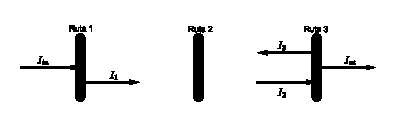
\includegraphics[scale=2]{images/tripleglazing.eps}
\caption{Visualisering av variabelnamnen använda vid härledning av reflektionsparametern för treglasfönster.}
\label{fig:tripleglazing}
\end{figure}

För en treglasruta gäller en något mer komplicerad annan reflektionsparameter. Betrakta figur \ref{fig:tripleglazing}. För $I_1$, den intensitet som släpps igenom första rutan, gäller att 

\begin{equation}
I_1=I_{in}\left( 1-a \right).
\end{equation}

På grund av en oändlig följd av reflektioner, även från den del av $I_3$ som passerar ruta 2 igen, blir $I_2 = \left( 1-a \right) I_1 \sum_{n=0}^{\infty} a^{2n} + a \left( 1-a \right)^2 I_3 \sum_{n=0}^{\infty} a^{2n}$. Men samtidigt måste också $I_3 = aI_2\sum_{n=0}^{\infty} a^{2n}$ vilket, om $I_2$ bryts ut, ger att

\begin{equation}
I_2 = \frac{\left( 1-a \right) I_1 \sum_{n=0}^{\infty} a^{2n}}{1-\left( 1-a \right)^2a^2\left(\sum_{n=0}^{\infty} a^{2n}\right)^2}.
\end{equation}

Detta tillsammans med det faktum att 

\begin{equation}
I_{ut} = \left( 1-a \right)I_2\sum_{n=0}^{\infty} a^{2n}
\end{equation}

ger, då dessa tre samband kombineras, att

\begin{equation}
I_{ut} = \frac{\left( 1-a \right)^3\left( \sum_{n=0}^{\infty} a^{2n}\right)^2}{1-\left( 1-a \right)^2a^2\left(\sum_{n=0}^{\infty} a^{2n}\right)^2}I_{in}.
\end{equation}

Notera nu att $\sum_{n=0}^{\infty} a^{2n} = \frac{1}{1-a^2}$ på grund av geometriska seriers egenskaper. Sätt in detta och förenkla så fås tillslut att

\begin{equation}
I_{ut} = \frac{\left( 1-a \right)^3}{\left(\left( 1-a^2\right)^2 - \left(1-a\right)^2 a^2\right)}I_{in} = 0,75 \cdot I_{in}
\end{equation}

då $a=0.1$.
